%!TEX root = ./document.tex

\section{Results}
\label{sec:Results}

We have generated heatmaps of averaged network dynamics that showcase general patterns for size-$n$ networks across the full spectrum of edge connection probabilities and degrees of symmetry. Utilizing these heatmaps, we can see a distinct zone of phase transition where the dynamics go from coalescing to a fixed point to exhibiting strongly chaotic behavior.\sidenote{It should be noted that chaotic behavior persists for longer for larger $n$ graphs.}


\subsection{Undirected Graphs}%
\label{sub:Undirected Graphs}

Additionally, we have also identified that for networks of increasing size $n$, $n\to\infty$ results in the expected number of any fixed $k$-size clique going to 0, $\sigma_k \to 0$.

The main approach utilized requires that we can identify the expected number of maximal cliques for any set of parameters $p$ and $q$. The expected number of maximal cliques is given by
\begin{align}
    \label{eq:e of max}
    \E_u[\mbox{maximal } \sigma_k] = \binom{N}{k}p^{\binom{k}{2}}
\end{align}
where $p$ is the probability of an edge between any two vertices in the network.\sidenote{I believe this might need some refinement.}
Additionally, the probability that a clique is maximal is given by
\begin{align}
    \label{eq:p max undirected}
    \PP_u{(\sigma_k \mbox{ is maximal}|\sigma_k \mbox{ exists})} = (1-p^k)^{N-k}.
\end{align}

Together, these two gives us the expected number of maximal cliques in any $N$-size undirected graph. The scheme for a directed graph is a little more complicated, but arises naturally.

\subsection{Directed Graphs}%
\label{sub:Directed Graphs}

First, we consider the expected number of maximal cliques. Instead of looking for general edge generation probability, we now look specifically at
%  nerd -ella
the probability that a bidirectional edge is generated, $pq$. So, the expected number of maximal cliques is given by
\begin{align}
    \label{eq:e of max directed}
    \E_d(\mbox{maximal } \sigma_k) = \binom{N}{k}pq^{\binom{k}{2}}.
\end{align}
Similarly, in order to find the probability that any $k$-clique is maximal, recall that we are essentially finding the complement of the probability that it is \textit{not} maximal. That is, we require the probability that the clique has any targets. Thus, we identify the probability of there existing a feed-forward edge to a vertex outside of the clique, $p \left(\frac{1-q}{2} \right)$ and $pq$. So,
\begin{align}
    \label{eq:p max directed}
    \PP_d(\sigma_k \mbox{ is maximal}|\sigma_k \mbox{ exists}) = \left[ 1- \left(pq + p   \left(\frac{1-q}{2} \right) \right)^k \right]^{N-k}.
\end{align} 
Moving forward, unless otherwise specified, we will always refer to the probabilities described for directed graphs.

The expected number of maximal cliques for an $N$-size network is given by the expected number of maximal cliques multiplied by the probability that any given clique is maximal given that it exists.
\begin{gather}
    \label{eq:expected max directed}
    \E_d \cdot \PP_d = \binom{N}{k}pq^{\binom{k}{2}} \left[ 1- \left(pq + p   \left(\frac{1-q}{2} \right) \right)^k \right]^{N-k}.
\end{gather}

\subsection{Numerical Results}%
\label{sub:Numerical Results}

Detailed below are the numerical methods used and their resulting simulations. These are the grounds that spurred the main goal\sidenote{Change to result once done!} of the paper.

To generate dynamics for individual graphs, we used a standard iterative method for numerically solving PDEs.
\begin{figure}[h]
     \centering
     \begin{subfigure}{0.45\textwidth}
         \centering
         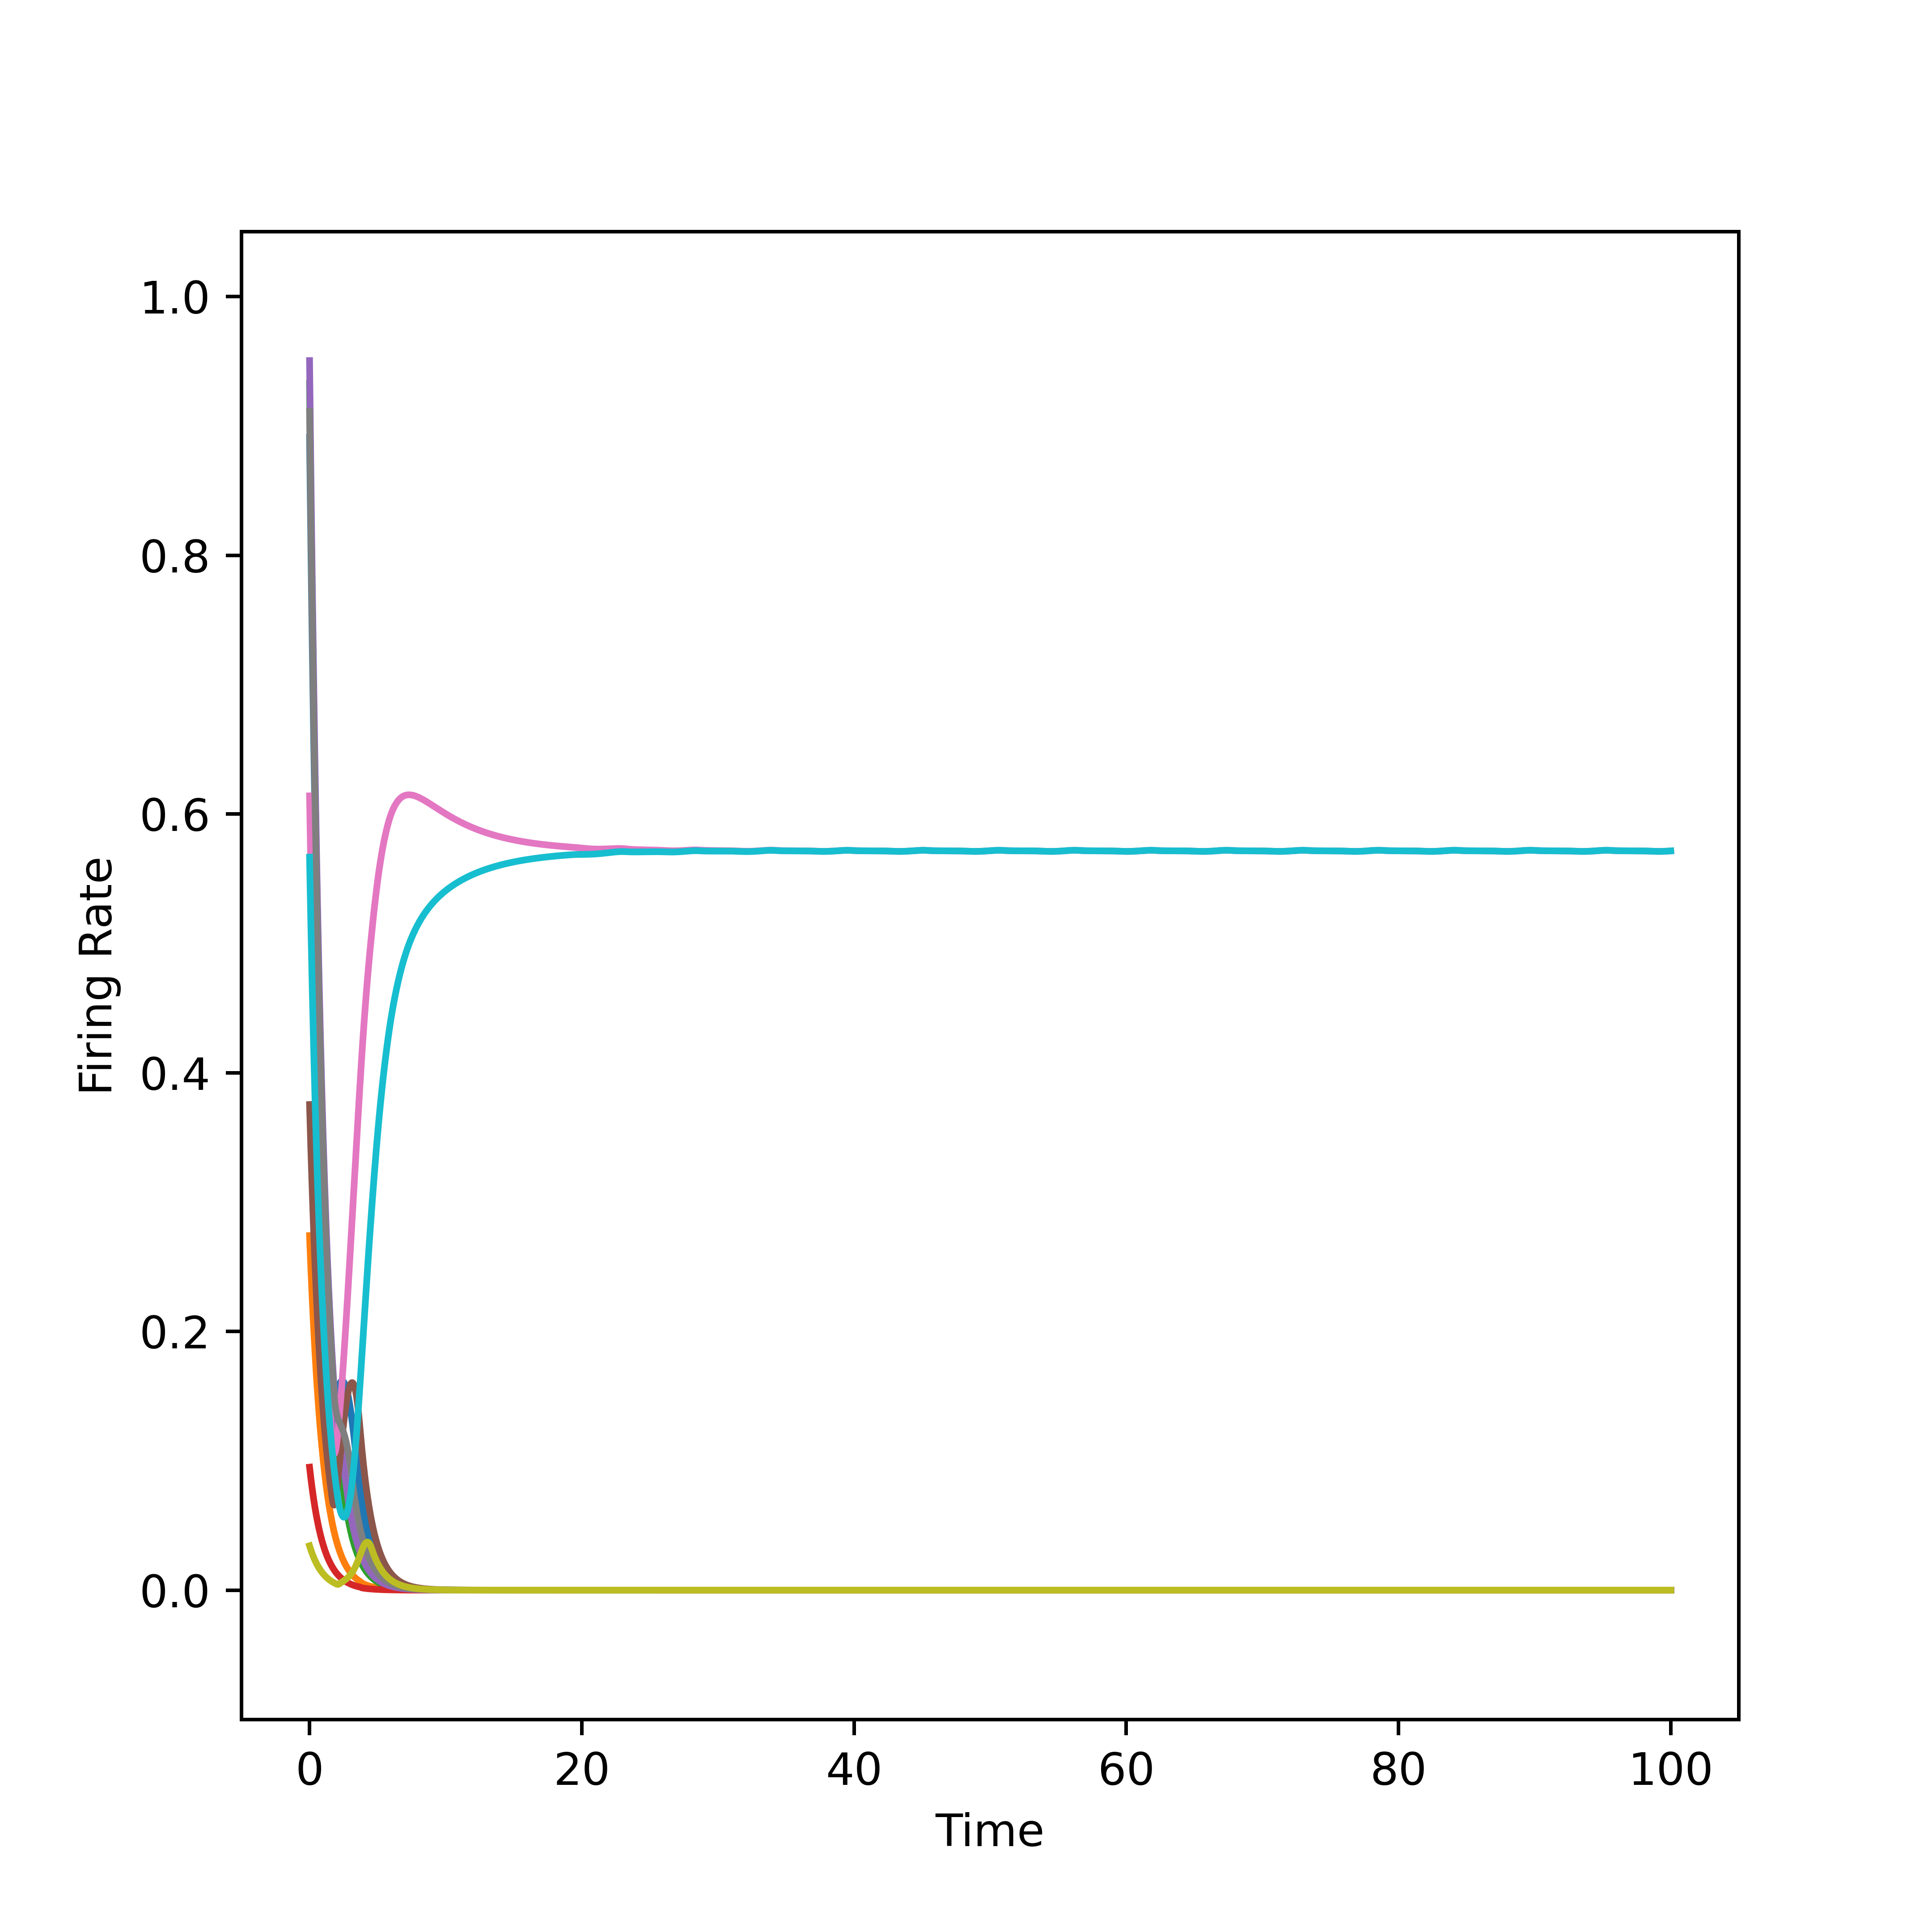
\includegraphics[width=\linewidth]{./Figures/Matrix Size 10 Symmetry 0.100 0.6 0.1 12.png}
         \label{fig:1a}
     \end{subfigure}
     \begin{subfigure}{0.45\textwidth}
         \centering
         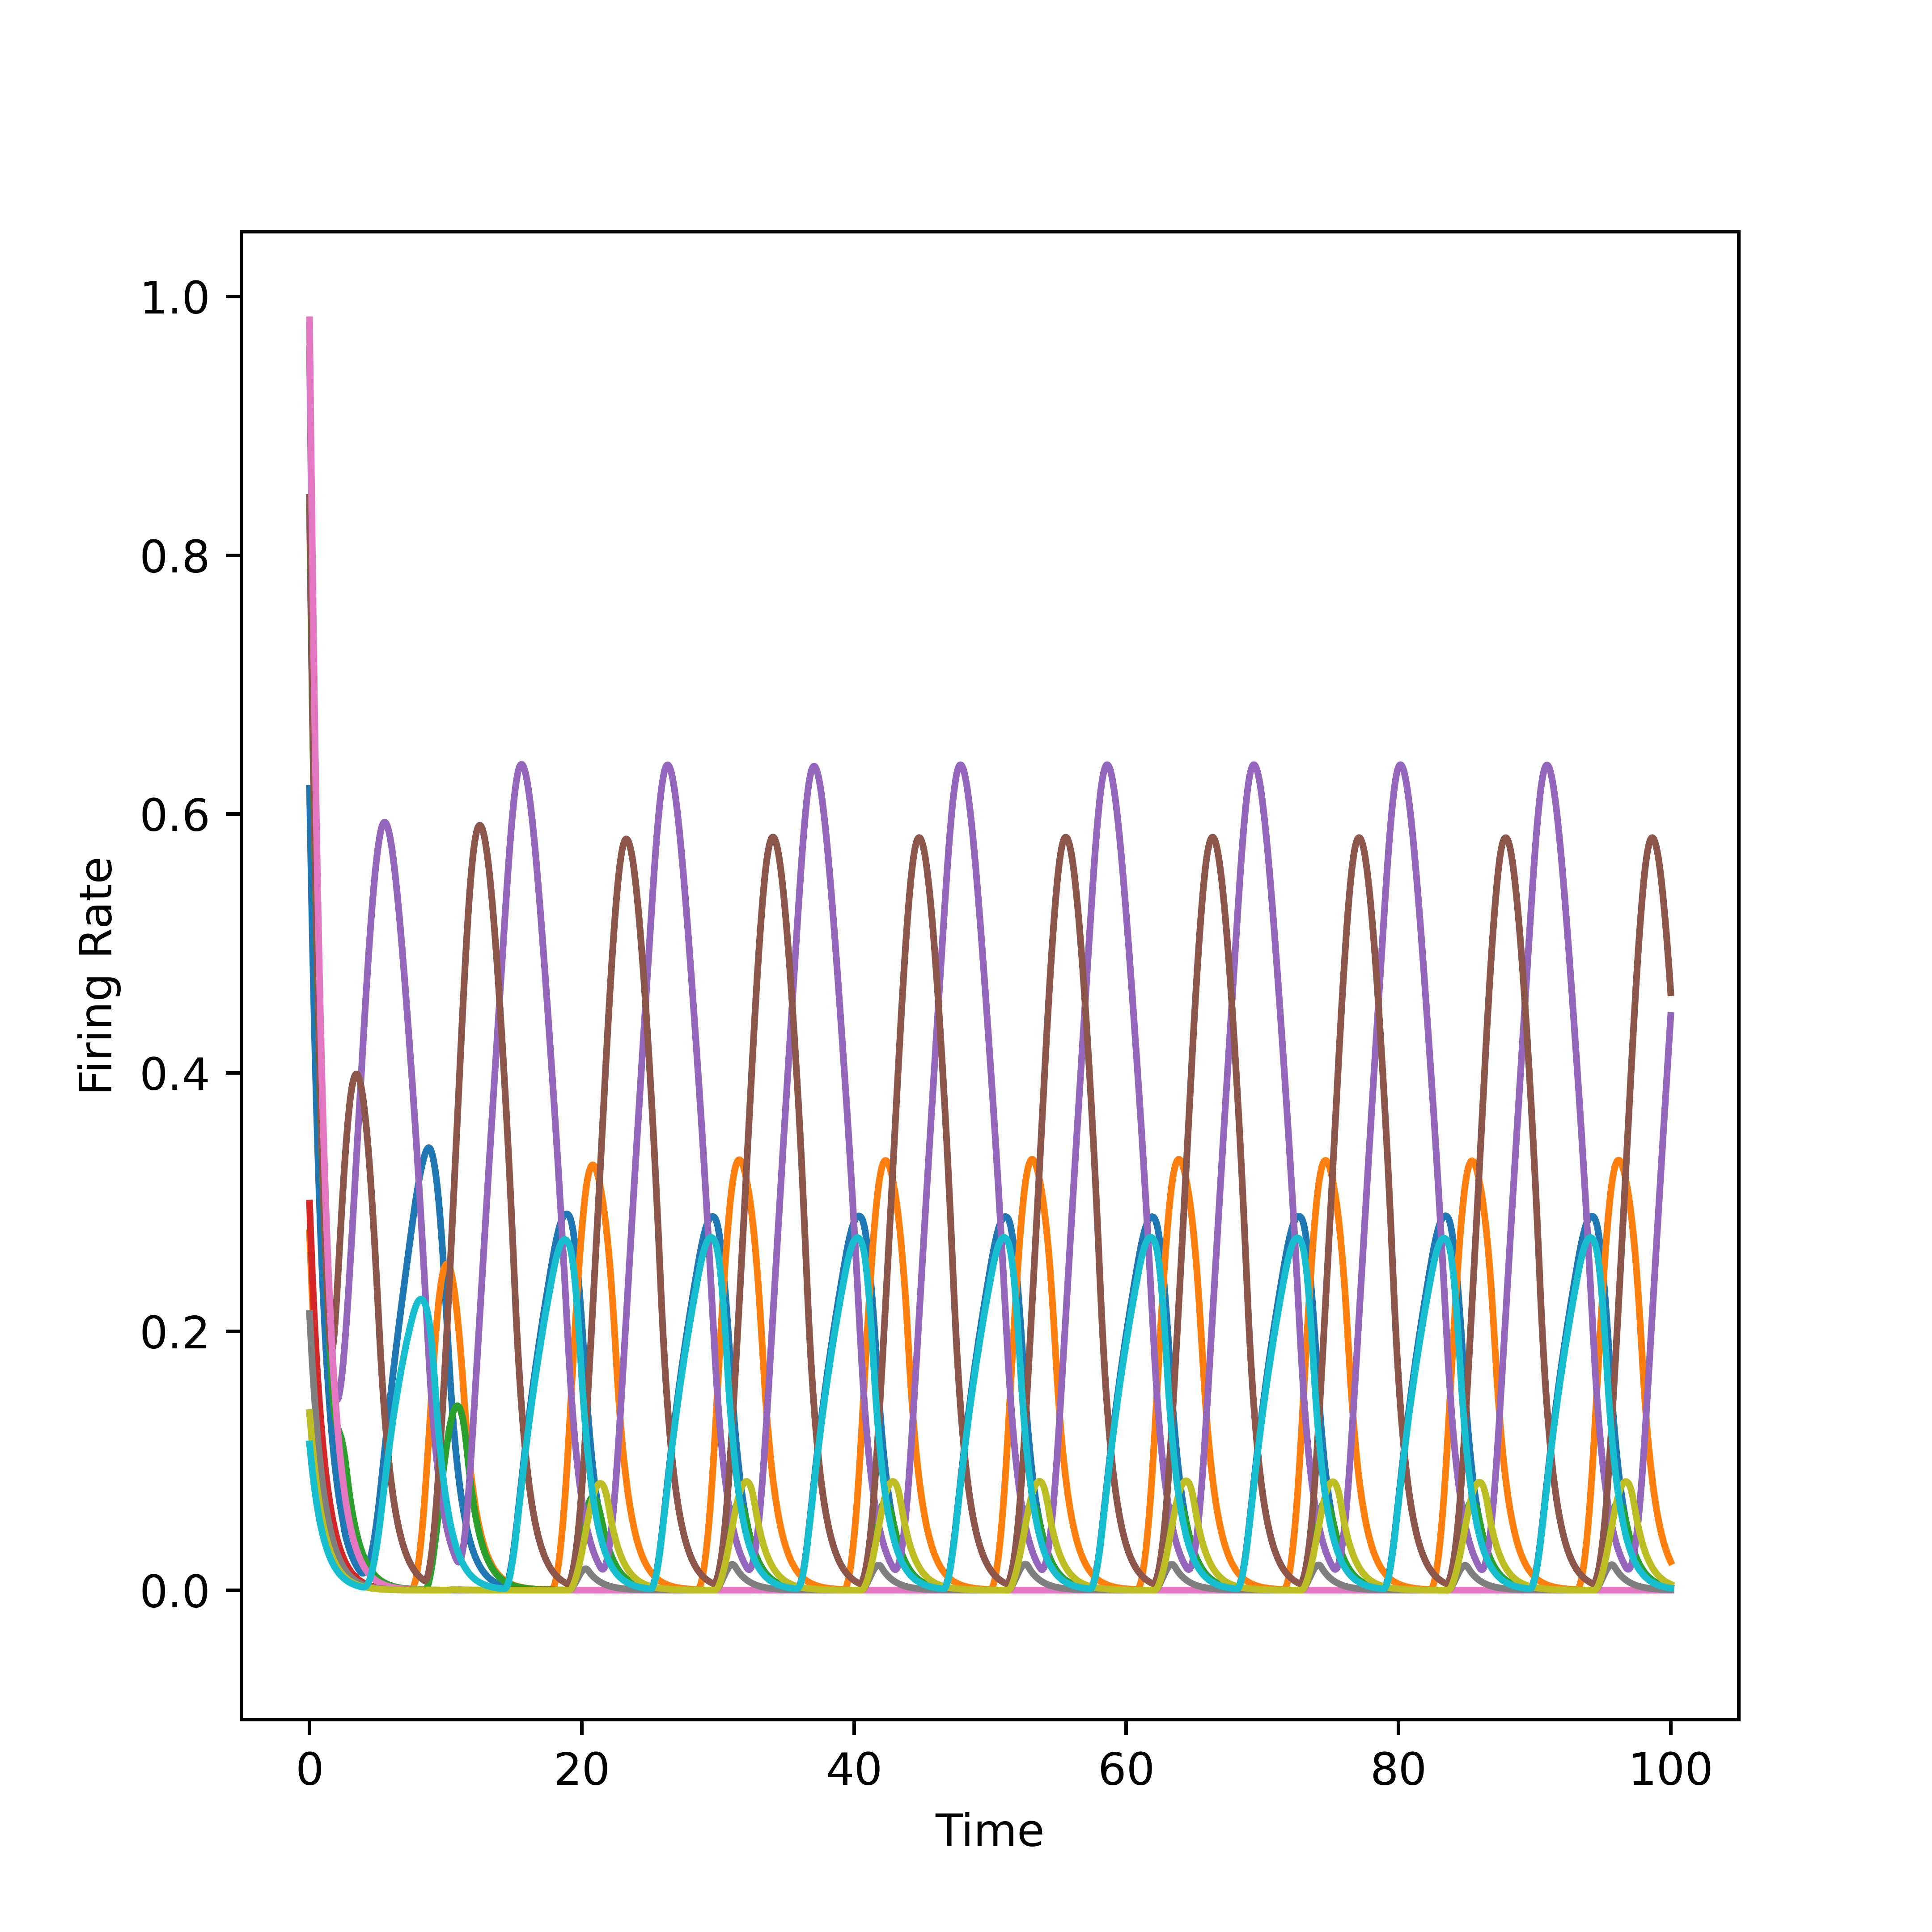
\includegraphics[width=\linewidth]{./Figures/Matrix Size 10 Symmetry 0.100 0.6 0.1 13.png}
         \label{fig:1b}
     \end{subfigure}
     \caption{Two 15-networks demonstrating different behavior despite having the same parameters. $N=15, p=0.6, q=0.1$. This highlights the variance in network dynamics, even in small networks. As network size is increased, outliers are less likely to occur, but coalescence to a steady state is much slower.}
     \label{fig:1}
\end{figure}

Accurate simulation of network dynamics means that we may average the behavior of randomly-generated networks across the entire spectrum of symmetry-edge connection values. To do this, we simply simulate the dynamics of networks with specific parameters multiple times in order to generate heatmaps that indicate how likely a specific pair of parameters is to result in a fixed point. We detect fixed points by numerically computing the derivatives at the final point in time.

\begin{figure}[h]
     \centering
     \begin{subfigure}{0.45\textwidth}
         \centering
         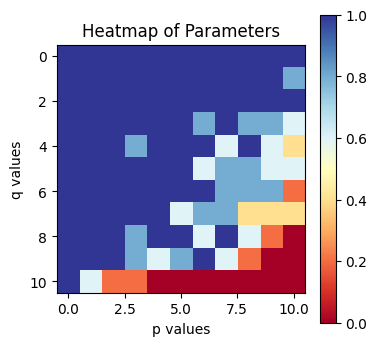
\includegraphics[width=\linewidth]{./Figures/size 30 heatmap.png}
         \label{fig:1a}
     \end{subfigure}
     \begin{subfigure}{0.45\textwidth}
         \centering
         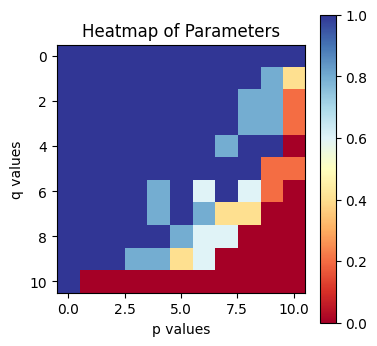
\includegraphics[width=\linewidth]{./Figures/size 100 heatmap.png}
         \label{fig:1b}
     \end{subfigure}
     \caption{Averaged heatmaps for a 30-network and a 100-network. Heatmaps were averaged over 7 trials. Red regions are more likely to coalesce to a limit cycles and blue regions are more likely to coalesce to a fixed point. One can clearly see a distinct zone of phase transition where firing rate trajectories ``shift'' to the other steady state. As network size grows, the phase transition becomes more prominent and pairs of parameters become more ``patterned''.}
     \label{fig:1}
\end{figure}

\section{Methods and Proofs}
\label{sec:Methods and Proofs}

